\documentclass[a4paper]{article}
\usepackage[utf8]{inputenc}
%% \usepackage[demo]{graphicx}
\usepackage[pdfborder={0, 0, 0}, colorlinks=true]{hyperref}

\usepackage{tikz, floatrow, pgfplots, enumitem, mathtools, tikz-uml, amsmath, bm}
\usetikzlibrary{positioning, shapes}

\newfloatcommand{capbtabbox}{table}[][\FBwidth]

\newcommand*\circled[1]{\tikz[baseline=(char.base)]{
    \node[shape=circle,draw,inner sep=1.5pt] (char) {#1};}}

\title{OpenPose picture}
\author{Bård-Kristian Krohg \\ \texttt{baardkrk@student.matnat.uio.no}}

\begin{document}
\maketitle


%% \begin{figure}
%%  \centering
\begin{figure}
  \begin{floatrow}
    \ffigbox{
      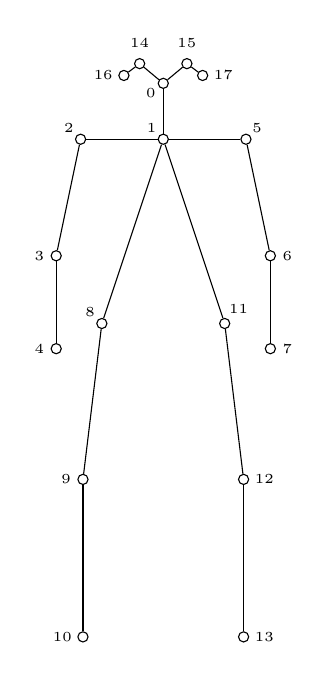
\begin{tikzpicture}[
          every node/.style={draw,circle,minimum size=.06cm, inner sep=1.3pt}
        ]
        \tiny
        %% \draw[help lines, step=5mm, gray!20] (-4,-4) grid (3,4);
        
        \node[label={[label distance=-.2mm]200:{0}}] (nose) at (0,3.25) {};
        \node[label={[label distance=-.2mm]140:{1}}] (neck) at (0,2.54) {};
        
        \node[label={[label distance=-.1mm]90:{14}}] (reye) at (-.3,3.5) {};
        \node[label={[label distance=-.1mm]90:{15}}] (leye) at (.3,3.5) {};

        \node[label={[label distance=-.1mm]180:{16}}] (rear) at (-.5,3.35) {};
        \node[label={[label distance=-.1mm]0:{17}}] (lear) at (.5,3.35) {};

        \node[label={[label distance=-.2mm]140:{2}}] (rshoulder) at (-1.05,2.54) {};
        \node[label={[label distance=-.2mm]50:{5}}] (lshoulder) at (1.05,2.54) {};
        
        \node[label={[label distance=-.1mm]180:{3}}] (relbow) at (-1.36,1.06) {};
        \node[label={[label distance=-.1mm]0:{6}}] (lelbow) at (1.36,1.06) {};

        \node[label={[label distance=-.1mm]180:{4}}] (rwrist) at (-1.36,-.12) {};
        \node[label={[label distance=-.1mm]0:{7}}] (lwrist) at (1.36,-.12) {};

        \node[label={[label distance=-.2mm]140:{8}}] (rhip) at (-.78,.2) {};
        \node[label={[label distance=-.2mm]50:{11}}] (lhip) at (.78,.2) {};

        \node[label={[label distance=-.1mm]180:{9}}] (rknee) at (-1.02,-1.78) {};
        \node[label={[label distance=-.1mm]0:{12}}] (lknee) at (1.02,-1.78) {};

        \node[label={[label distance=-.1mm]180:{10}}] (rankle) at (-1.02,-3.78) {};
        \node[label={[label distance=-.1mm]0:{13}}] (lankle) at (1.02,-3.78) {};

        %% \draw[blue] (0,0) circle [radius=.06cm];

        \draw (nose) -- (neck);
        \draw (reye) -- (nose); \draw (leye) -- (nose);
        \draw (reye) -- (rear); \draw (leye) -- (lear);
        
        \draw (neck) -- (rshoulder); \draw (neck) -- (lshoulder);
        \draw (neck) -- (rhip); \draw (neck) -- (lhip);

        \draw (rshoulder) -- (relbow); \draw (lshoulder) -- (lelbow);
        \draw (rwrist) -- (relbow); \draw (lwrist) -- (lelbow);

        \draw (rhip) -- (rknee); \draw (lhip) -- (lknee);
        \draw (rknee) -- (rankle); \draw (lknee) -- (lankle);
      \end{tikzpicture}
    }
    {
      \label{fig:openpose_skeleton}
      \caption[Numbering for OpenPose's keypoint markers]{Numbering for OpenPose's keypoint markers.}
    }
    %% \end{figure}
    %% \begin{table}
    \capbtabbox{
      \begin{tabular}[H]{r l}
        ID & Name \\ \hline
        0  & Nose \\
        1  & Neck \\
        2  & Right Shoulder \\
        3  & Right Elbow \\
        4  & Right Wrist \\
        5  & Left Shoulder \\
        6  & Left Elbow \\
        7  & Left Wrist \\
        8  & Right Hip \\
        9  & Right Knee \\
        10 & Right Ankle \\
        11 & Left Hip \\
        12 & Left Knee \\
        13 & Left Ankle \\
        14 & Right Eye \\
        15 & Left Eye \\
        16 & Right Ear \\
        17 & Left Ear \\
        \hline
      \end{tabular}
    }{
      \label{tab:openpose_body_ids}
      \caption[IDs for OpenPose keypoint markers]{IDs for OpenPose's keypoint markers.}
    }
  \end{floatrow}
\end{figure}
%% \end{table}

\begin{figure}
  \centering
  \begin{floatrow}
    \ffigbox[.3\textwidth]{
      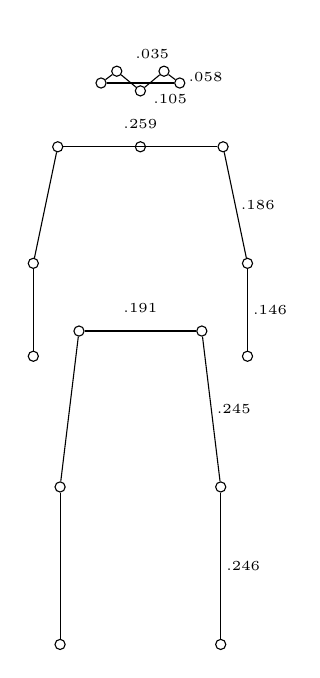
\begin{tikzpicture}[
          every node/.style={draw,circle,minimum size=.06cm, inner sep=1.3pt}
        ]
        \tiny
        %% \draw[help lines, step=5mm, gray!20] (-4,-4) grid (3,4);
        
        \node (nose) at (0,3.25) {};
        \node (neck) at (0,2.54) {};
        
        \node (reye) at (-.3,3.5) {};
        \node (leye) at (.3,3.5) {};

        \node (rear) at (-.5,3.35) {};
        \node (lear) at (.5,3.35) {};

        \node (rshoulder) at (-1.05,2.54) {};
        \node (lshoulder) at (1.05,2.54) {};
        
        \node (relbow) at (-1.36,1.06) {};
        \node (lelbow) at (1.36,1.06) {};

        \node (rwrist) at (-1.36,-.12) {};
        \node (lwrist) at (1.36,-.12) {};

        \node (rhip) at (-.78,.2) {};
        \node (lhip) at (.78,.2) {};

        \node (rknee) at (-1.02,-1.78) {};
        \node (lknee) at (1.02,-1.78) {};

        \node (rankle) at (-1.02,-3.78) {};
        \node (lankle) at (1.02,-3.78) {};

        %% \draw[blue] (0,0) circle [radius=.06cm];

        \draw (reye) -- (nose); \draw (leye) -- node[above, draw=none, inner sep=2.5pt] {.035} ++(nose);
        \draw (reye) -- (rear); \draw (leye) -- node[right, draw=none, inner sep=4.3pt] {.058} ++(lear);

        \draw (rear) -- node[below right, draw=none, xshift=5pt] {.105} ++(lear);
        
        \draw (lshoulder) -- node[above, draw=none] {.259} ++(rshoulder);

        \draw (rshoulder) -- (relbow); \draw (lshoulder) -- node[right, draw=none] {.186} ++(lelbow);
        \draw (rwrist) -- (relbow); \draw (lwrist) -- node[right, draw=none] {.146} ++(lelbow);

        \draw (rhip) -- (rknee); \draw (lhip) -- node[right, draw=none] {.245} ++(lknee);
        \draw (rknee) -- (rankle); \draw (lknee) -- node[right, draw=none] {.246} ++(lankle);

        \draw (rhip) -- node[above, draw=none] {.191} ++(lhip);
      \end{tikzpicture}
    }
    {
      \label{fig:constrained_lengths}
      \caption[Constrained Lenghts]{Constrained lengths\protect\footnotemark.}
    }
    %% \end{figure}
    %% \begin{table}
    \capbtabbox{
      \begin{tabular}[H]{|r l|l|c|c}
        ID & Limb & Model & Pair & $\pm\bm{t}$ \\
        \hline
        0 & Left arm & .186 & 5 -- 6 & .05 \\
        1 & Left forearm & .146 & 6 -- 7 &.05 \\
        2 & Right arm & .186 & 2 -- 3 & .05\\
        3 & Right forearm & .146 & 3 -- 4 & .05\\
        4 & Hip & .191 & 8 -- 11 & .06\\
        5 & Left thigh & .245 & 11 -- 12 & .07 \\
        6 & Left leg & .246 & 12 -- 13 & .07 \\
        7 & Right thigh & .245 & 8 -- 9 & .07 \\
        8 & Right leg & .246 & 9 -- 10 & .07 \\ \hline
      %%   $\lvert Right shoulder - Right elbow\rvert = \lvert Left shoulder - Left elbow \rvert$
      %%   \hline
      \end{tabular}
    }{
      \label{tab:constrain_rules}
      \caption[Anthropometry constrain rules]{Constrain rules for correct anthropometry. (Note that the anthropometry for the head and shoulders are not yet implemented.)}
    }
  \end{floatrow}
\end{figure}


%% \begin{figure}
%%   %\tdplotsetmaincoords{70}{110}
%%   \begin{tikzpicture} \begin{axis}[view/h=-30] \addplot3[ surf, %shader=interp,
%%         shader=flat, samples=50, domain=-3:3,y domain=-2:2] {sin(deg(x+y^2))}; \end{axis} \end{tikzpicture}

%%   \label{fig:point_probability}
%%   \caption[Probability of picking points for 3D estimation]{The probability of picking points to fit the 3D line between keypoint A and B.}
%% \end{figure}

%% \footnotetext{http:\/\/openlab.psu.edu\/tools\/proportionality\_constants.htm}
\footnotetext{\url{http://openlab.psu.edu/tools/proportionality_constants.htm}}

\section{Placement Algorithm}
\begin{enumerate}[label=\protect\circled{\footnotesize\arabic*}]
\item Arrange Best matching limbs based on the score of the two connecting keypoints.
\item Select the \emph{N} best matching limbs and calculate a scale \emph{S} based on them.
\item Create vectors for all limbs under a certain threshold \emph{T}.
\item Shift keypoints under a certian threshold \emph{T} along the beam created by the 2D keypoint and the camera center. (increase Z and recalculate X and Y)
\item If the depth information at a keypoint is very uncertain, we should also rely on the depth information along the limb, flowing from the most certain keypoint to the least certain keypoint. This will also give us a vector along which we can place the point.
\item Calculate the difference in size between the observed limbs $\mathbf{L}_{v}$ and the model limbs $\mathbf{M}_{v}$\footnote{change the name of these variables}. The error \emph{E} is then given by
  \[
  E = \sum_{i=0}^{K}\lvert \mathbf{L}_{v}(i)\cdot s(i)^3 - \mathbf{M}_{v}(i)\rvert
  \]
\end{enumerate}

\textbf{Limb scores} \\
When doing this it is important that we also check how similar the values are to each other. If they have a large gap, but high average, we don't want them amog the high scoring results.
\[
\frac{a + b}{2} \cdot \lfloor a, b\rfloor^{3} \quad\mid\quad a,b \in [ \, 0, 1 ] \,
\]

\textbf{Scale (height)}
If we have the vector of limb scores \emph{S} and the vector of limb lengths \emph{L}, desired limb lengths \emph{D} we get the scale/height \emph{w} by taking the weighted averages of each observed limb.
\[
w = \frac{\sum_{i=0}^n\frac{L_{i}}{D_{i}}S_{i}}{\sum_{i=0}^{n}S_{i}}
\]

Doing it simple.

For each limb under the \emph{threshold}:\\
Use S to get the scale of what the current limb's length \emph{should} be.\\
create the ``vector'' of the limb to get the 3D direction in which to move/place the keypoint.\\
$\rightarrow$ Creating the vector, search along the limb in the depth image. If we get to an edge, use the previous points to create the 3D vector (line) using RANSAC.

The limbs are stored as tuples:
\texttt{\{<score>, <length>\}}

\textbf{Creating the model parameters} \\
For each person we need a set of model parameters to predict the 3D location of each keypoint. These parameters consist of \textbf{t} -- a set of numbers representing the leeway we give to each limb in relation to the model. The formula we get for fitting the human model to the observed locations is
\[
Error = \sum_{all limbs} (scale (model\_length + \textbf{t}_{i}) - actual\_length) \cdot score\_of\_observed\_keypoint
\]
\[
E = \begin{bmatrix}
  S \begin{bmatrix}
    ML + \textbf{t}_{i} \\ \vdots
  \end{bmatrix} -
  \begin{bmatrix}
    ac\_L \\ \vdots
  \end{bmatrix}

\end{bmatrix}^{T}\cdot
\begin{bmatrix}
  score \\ \vdots
\end{bmatrix}
\]

where we minimize the error by changing \textbf{r} and \emph{scale}. If we already have calculated a previous set of parameters we should take this previous model into consideration. Therefore each model should be given a score, based on how ``old'' it is, the score of the parameters used in creating the model (the keypoint score for the N limbs used to create the model). The ``old'' part can be fixed by increasing the score after each iteration.

Each person should therefore have their own variables with \textbf{t}, \emph{scale} and \emph{current\_score}.

After we now have the predicted lengths for each limb, we can estimate the 3D positions for the different keypoints. Here, we should also have the previous or predicted keypoints (Kalman filter) to smooth the movement of the person. This should also be weighted however, because an observation with high score should trump a prediction any time. However, if we have no observation, we can use the predicted position from the previous frame to also track non-observed limbs.
We should also include a score for this, so we know which positions have had the most modification by this algorithm. This can be an input to the activity recognition algorithm to possibly account for wrong predictions and other noise. 





\section{The Program UML}

\begin{tikzpicture}
  \begin{umlpackage}{rgbd-pose}
    \umlclass{Person}{
      coordinates[18] : geometry\_msgs::Point \\
      coordinates2d[18] : geometry\_msgs::Point \\
      bpscore[18] : float \\

      br : tf::TransformBroadcaster \\
      transform : tf::Transform \\

      
    }{
      -publish\_line\_strip(a, b : geometry\_msgs::Point, body\_part : int, marker\_pub : ros::Publisher*) \\
      draw\_skeleton(*marker\_pub : ros::Publisher) : void \\
      set\_id(\_id : int) : void \\
      get\_id(); : int \\
      set\_score(body\_part : int, score : float) : void \\
      get\_score(body\_part : int) : float \\
      set\_coordinate(body\_part : int, point : geometry\_msgs::point) : void \\
      get\_coordinate() : geometry\_msgs*
    }
  \end{umlpackage}
\end{tikzpicture}

\section{rgbd-pose}

\subsection{Person}
Storage class for each person object. Every person has an \emph{ID} and a set of \emph{coordinates} (2d and 3d). Each person also has a \emph{base\_frame} which is a string. The person class is able to publish line strips between each of it's keypoints, and thus draw itself in rviz.
\subsubsection{ID} is a unique identifier for each person, and is an integer for the moment.
\subsubsection{Coordinates} we have two separate coordinate arrays, as one stores the 2D image positions of each keypoint, and the other stores the 3D calculated positions of each keypoint. The 3D coordinates are subject to change when we constrain the pose using the \texttt{pose\_estimator} class.
\subsubsection{base\_frame} tells us what this persons coordinates are calculated from. We can then translate the persons coordinates to other ROS frames, as long as we know their relation to this \emph{base\_frame}.

\subsection{pose\_estimator}
A utility class for gathering all functions that helps us estimate the 3D pose of the persons. This class also runs the openpose program on provided frames. We create this object only one time, but it is updated with new \emph{depth frames} and \emph{frames}. This is because OpenPose runs on individual frames, and not on video sequences.
In addition the \texttt{pose\_estimator} class has parameters for the \emph{focal length} and the \emph{pixel center} of the camera model for the frames. We need this when we place the points into 3D space. 

\section{Notes}

\textbf{Time sync for ROS-TMS:} do the same as in ``Multiple Depth Cameras Calibration and Body Volume Reconstruction for Gait Analysis''. (Separate computers are synched with NTP, send information to central server. This runs.. wait there is a problem with subscribing to topics with ROS... ALTHOUGH, if the separate computers are good enough, they could calculate the 3D positions and publish q

\textbf{some ideas for abstract:} The easiest way to diagnose a patient is to go to them. .. many patients .. no time .. better with routine checks .. 

Hjemmesykepleien sliter med ufaglærte. derfor bedre med et automatisk system som kan hjelpe til med å kjenne igjen de viktigste faresignalene hjemme. Et ``alt i ett'' system som kan passe på tabeletter osv i tillegg. 
\listoffigures
\listoftables

\section{Solving multiple view stereo}


\end{document}
